\subsubsection{Manpower}

This section will address the outline for the current available manpower of the IRISC team, this includes the tasks assigned to each member and the hours per week that each team member will dedicate to the project.

\begin{longtable}{m{0.25\textwidth} | m{0.6\textwidth} | m{0.1\textwidth}}
	\textbf{Team Member} & \textbf{Tasks Description} & \textbf{hours/week} \\ \hline
	Diego Talavera  & \textbf{Team Manager}. Was in charge of the management of the resources of the team and supervising the overall progress of the activities. Also provided technical support to the Mechanical Engineering branch. &  30-40 \\ \hline
	Niklas Ulfvarson & \textbf{ Vice Team Manager \& Ground Station System \& Star Tracker}. Was in charge of developing the software needed for monitoring and controlling (if needed) the experiment from the ground as well as to visualize the data received by the telemetry system. Also implemented the star tracker for attitude determination, and assisted with management and supervision of the team. & 30 \\ \hline
	Kimberly Steele & \textbf{Astronomy \& Data analysis}. Was in charge of the target selection and provide the technical requirements to achieve proper imaging of said targets. Was also involved in the data analysis after the BEXUS flight campaign and as well minor tasks for the outreach campaign. & 30 \\ \hline
	Jack Hooper & \textbf{Thermal Engineering}. Was to ensure that the thermal requirements for the proper functioning of the experiment during the ascent, flight and descent phases were met. This included design and selection of active/passive heating and cooling where needed and recommendations regarding materials. & 25 \\ \hline
	Elrick Weterings & \textbf{Embedded systems}. Was in charge of the design and selection for the electronic components including sensors and motors used to stabilize the telescope. He was also in charge of designing the necessary printed circuit boards (PCBs). & 30 \\ \hline
	Sabina Bj{\"o}rk & \textbf{Energy Technologies}. Was to ensure that the power required was delivered to all the subsystems during all phases of the experiment. & 25-35 \\ \hline
	Anja M{\"o}slinger & \textbf{Control System}. Was responsible for the development and testing of the control loop necessary to stabilize the telescope to the required degree of accuracy. & 30 \\ \hline
	Adam Smialek & \textbf{Control system}.  Helped in the development of the control loop, including the code testing and implementation. He also helped with some tasks in the Outreach branch, like the fundraising campaign. & 20 \\ \hline
	Harald Magnusson & \textbf{Onboard data}. Was in charge of the development of the software necessary by the experiment in order to function correctly, including data processing, handling and delivery. & 30 \\ \hline
	William Eriksson & \textbf{Onboard data}. Was also involved in the development of the software required on board of the experiment, this also included data processing and handling, telemetry, etc. & 30 \\ \hline
	Jon Mihkkal Inga & \textbf{Mechanical Engineering}. Designed the mechanical setup of the experiment, including FEM analysis and its construction. & 20 \\ \hline

\end{longtable}

\newpage
\begin{landscape}
	\begin{figure}[H]
		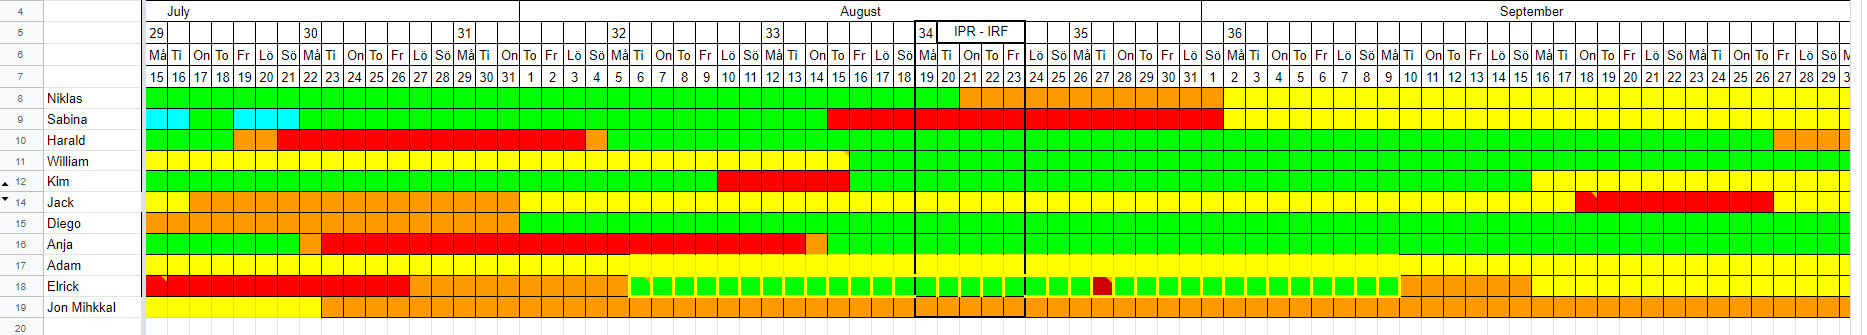
\includegraphics[scale=1.2]{3-project-planning/img/availability.png}
		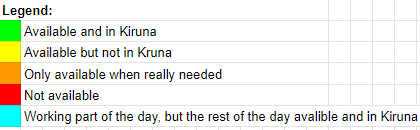
\includegraphics[scale=1.2]{3-project-planning/img/Availability_legend.png}
		\caption{Availability chart of the team members}
	\end{figure}
\end{landscape}

\newpage
\subsubsection{Budget}
\label{sec:3.2.2}

%This table is fancy and will line up your decimal points, unlike the normal table, so it looks prettier :3
\begin{table}[H]
\centering
\begin{tabular}{|l|c|c|c|} 
\hline
Source & Amount (\euro) & Limitations   \\ 
\hline
Luleå University of Technology & 1000 & Hardware and travel \\
SNSA & 3000 & Hardware and travel \\
Crowdfunding Campaign & TBD & None \\
\hline
\textbf{Total projected income} & \textbf{4000} & \\
\hline
\bf{Total projected cost} & \bf{2681.5} & \\
\hline
\end{tabular}
\caption{Income and projected cost.}
\label{table:income-and-cost}
\end{table}

\raggedbottom
%This table is fancy and will line up your decimal points, unlike the normal table, so it looks prettier :3
\begin{table}[H]
\centering
\begin{tabular}{|c|d{2}|d{2}|}%{D{.}{.}{1}}
\hline

\textbf{Category} & \textbf{Total Mass [g]} & \textbf{Total Price [EUR]} \\ \hline
Structure & 5000 & 500 \\ \hline
Electronics Box &  2000 & 500 \\ \hline
Telescope & 5000 & 1500 \\ \hline
Cables and Sensors &  &  \\ \hline
Tools & - & TBD \\ \hline
Travel & - & TBD \\ \hline
Contingency & - & TBD  \\ \hline
{\textbf{Total without Error Margin}} & \textbf{} & \textbf{TBD} \\ \hline
Shipping Costs and Error Margin &  &  \\ \hline
{\textbf{Total with Error Margin}} & \textbf{} & \textbf{TBD} \\ \hline
\end{tabular}
\caption{Mass and Cost Budget.}
\label{table:mass-and-cost-budget}
\end{table}

\raggedbottom


\subsubsection{External Support}

\begin{itemize}
	\item Mr. Olle Persson. Provided help with getting access to some testing facilities as well as potential questions in the Mechanical Engineering branch of the project.
	\item Adam Burgasser, PhD. Helped us with the data analysis and interpretation after the flight with BEXUS.
	\item LUDD - Luleå Academic Computer Society. They provided the hosting to the official IRISC web page.
	\item GranaSAT, team from Bexus 19 which provided help with the attitude determination system.
\end{itemize}
